\chapter{Results}
\label{cha:chapter4}
In this section are shown the results obtained in different test. Divided in different steps thought the implementation of the modules in the vehicle such as, image processing off vehicle; first approach that cover the vehicle moving straight in the lane, positioned with an error on purpose, taking a curve. 

\section{Image Processing}
By the time the first tests were done the road was simulated using a black cardboard with white tape for the lines as shown in the Figure \ref{fig:StraightLane} and Figure \ref{fig:AngleLane}, but the measurements are not the same as mentioned in the Chapter \ref{cha:chapter 1} the width its smaller by 10 cm each side. The algorithm is robuts enough to identity the lines with the correct angle even with a strong exposition to light. The lane angle obtained using the line detection tells the user how disoriented the vehicle is from the lane it can tell that $lane\_angle<90 = disoriented to the left$ and $lane\_angle>90 = disoriented to the right$.
All the pictures were taken in using the Kinect cam from the vehicle. However, the process was performed in a computer aside from the vehicle.

    \subsection{Straight Lane}
    Here the vehicle was oriented in a parallel direction to the lane giving as an output a lane angle of 90 degrees.
    
    \begin{figure}[h]
    \centering
    \subfigure[Perspective Transform]{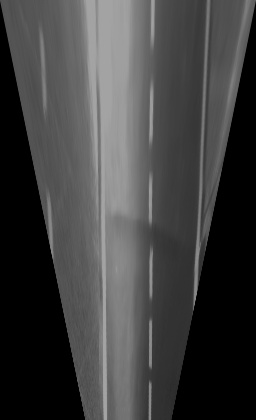
\includegraphics[width=35mm]{Figures/Results/StraightLine/Resultado_Warped2.jpg}}
    \subfigure[Angle]{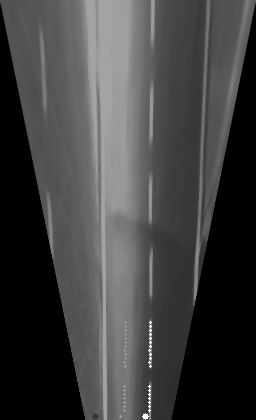
\includegraphics[width=35mm]{Figures/Results/StraightLine/Resultado_Puntos2.jpg}}
    \subfigure[Original]{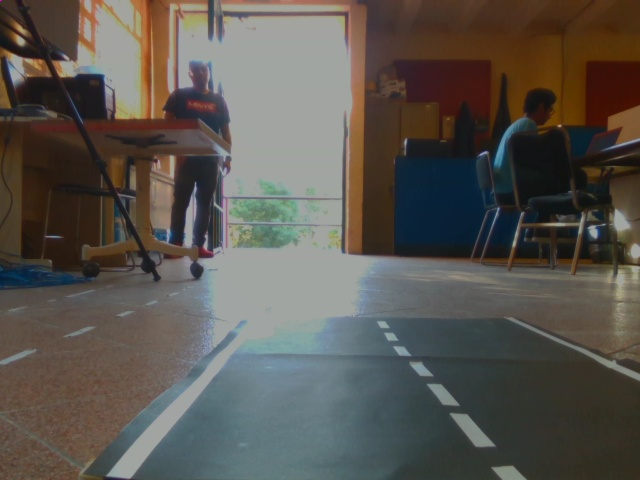
\includegraphics[width=75mm]{Figures/Results/StraightLine/Resultados2.jpg}}
    \caption{Straight Lane} \label{fig:StraightLane}
    \end{figure}
    
    
    \subsection{Angle Lane}
    Here the vehicle was oriented to the left side of the lane, expecting getting a lane angle below the 90 degrees. Giving as an output a result of 86 degrees.
    
    \begin{figure}[h]
    \centering
    \subfigure[Perspective Transform]{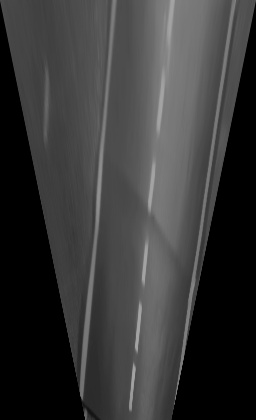
\includegraphics[width=35mm]{Figures/Results/AngleLine/Resultado_Warped1.jpg}}
    \subfigure[Angle]{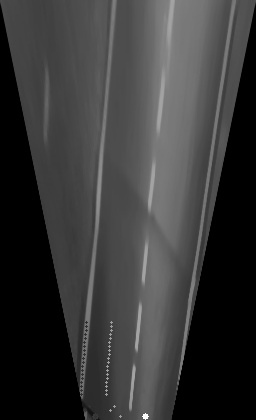
\includegraphics[width=35mm]{Figures/Results/AngleLine/Resultado_Puntos1.jpg}}
    \subfigure[Original]{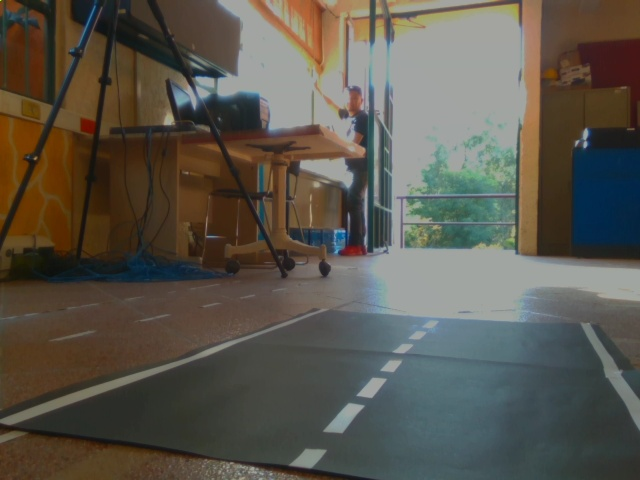
\includegraphics[width=75mm]{Figures/Results/AngleLine/Resultados1.jpg}}
    \caption{Angle Lane} \label{fig:AngleLane}
    \end{figure}

\section{First Approach}
A first approach was properly realized with a lane using the measurements previously mentioned in the Chapter \ref{cha:chapter 1} as well as a curve with the expected external radius. 
